\documentclass[conference]{IEEEtran}

\usepackage{amsmath,amssymb}
\usepackage{booktabs}
\usepackage{graphicx}
\usepackage{url}
\usepackage{xcolor}
\usepackage{listings}
\usepackage{hyperref}
\hypersetup{colorlinks=true,linkcolor=black,citecolor=black,urlcolor=blue}

\title{A Unified Image Restoration and Conditional Face-to-Sketch Studio Using Autoencoders, Mixture-of-Experts, and GANs}

\author{\IEEEauthorblockN{Assignment Implementation Report}
\IEEEauthorblockA{Generative AI Systems\\
2026}}

\begin{document}
\maketitle

\begin{abstract}
This paper presents an end-to-end image restoration and face-to-sketch system organized into four model workspaces. Task 1 uses a universal convolutional denoising autoencoder for clean, salt-and-pepper, Gaussian-blurred, and occluded images. Task 2 adds a corruption classifier and three independently trained specialists under hard routing. Task 3 replaces discrete selection with a differentiable soft mixture-of-experts containing an identity branch and three restoration experts. Task 4 uses a style-conditioned U-Net generator and PatchGAN discriminator for paired face-to-sketch synthesis on FS2K. Optuna is used to investigate the requested learning and architecture hyperparameters. Models are exported to ONNX and checked against ONNX Runtime. A React/Tailwind frontend, FastAPI inference service, and Docker Compose deployment complete the application architecture. The reported results are accompanied by explicit compute-budget limitations because the experiments were executed in a CPU-constrained development environment.
\end{abstract}

\begin{IEEEkeywords}
image restoration, denoising autoencoder, mixture-of-experts, conditional GAN, FS2K, ONNX Runtime, Optuna
\end{IEEEkeywords}

\section{Introduction}
Image restoration is not a single corruption problem. Sensor noise, blur, missing regions, and clean inputs require different inductive biases, while an application must expose one predictable inference interface. This project investigates four progressively more structured solutions: one universal restoration model, hard-routed specialists, a soft mixture-of-experts, and a conditional image-to-image GAN for face-to-sketch synthesis.

The implementation has two goals. First, each model must satisfy the architectural constraints of the assignment, including a real autoencoder bottleneck, explicit structural losses, learned routing, and learned style conditioning. Second, the research artifacts must be usable in an application: the models are exported to ONNX, inference is served through FastAPI, and the frontend presents the four workspaces through one React application.

\section{Related Work}
U-Net introduced encoder-decoder image translation with skip connections \cite{ronneberger2015unet}. Conditional adversarial image translation and PatchGAN-style local discrimination motivate the paired face-to-sketch design \cite{isola2017pix2pix}. The restoration losses use the L1 and structural similarity principles of SSIM \cite{wang2004ssim}. Mixture-of-experts models motivate separating routing from specialist computation, while the FS2K dataset provides paired photographs, sketches, annotations, and three sketch styles \cite{fan2022fs2k}.

\section{Dataset Preparation}
\subsection{Oxford-IIIT Pet}
Tasks 1--3 use the Oxford-IIIT Pet dataset. The official test split remains untouched. The official training portion is split into training and validation data using seed 42 and an 80/20 split. The corruption pipeline samples four equally likely input conditions during training: clean, salt-and-pepper noise, Gaussian blur, and rectangular occlusion. Validation and test corruption settings are deterministic and include low, medium, and high severity manifests.

The corruption settings are probability $0.03/0.08/0.15$ for salt-and-pepper noise, $(k,\sigma)=(3,0.7),(5,1.5),(7,2.5)$ for blur, and approximately $10\%,20\%,35\%$ coverage with one, two, and three masks for occlusion.

\subsection{FS2K}
Task 4 uses the official FS2K archive, which contains 2,104 paired photographs and sketches. The official definitions contain 1,058 training pairs and 1,046 test pairs. Fifteen percent of the official training portion is reserved for validation with seed 42, stratified by the three annotation style categories. The official test set is not used for training or hyperparameter selection. Photographs and sketches are resized to $128\times128$ while preserving each pair.

\section{Task 1: Universal Restoration}
\subsection{Architecture}
The universal model is a convolutional encoder-decoder. The encoder progressively reduces spatial resolution and increases channels. A convolutional bottleneck followed by adaptive pooling creates a genuine compressed representation. The decoder reconstructs an RGB image and uses a sigmoid output. No corruption label is provided to the model.

\subsection{Loss}
For clean target $x$ and prediction $\hat{x}$, the objective is
\begin{equation}
L_{\mathrm{universal}}=\alpha L_1(x,\hat{x})+(1-\alpha)(1-\mathrm{SSIM}(x,\hat{x})).
\end{equation}
SSIM is implemented with differentiable PyTorch local statistics rather than a detached evaluation-only metric.

\subsection{Optuna and Results}
Optuna investigated learning rate, batch size, bottleneck dimension, encoder channels, dropout, and $\alpha$. Three trials were completed at $64\times64$ with eight training batches and four validation batches per trial. The best configuration was learning rate $2.3689\times10^{-4}$, batch size 8, latent dimension 64, base channels 16, dropout 0.00618, and $\alpha=0.93646$. The best recorded validation loss was 0.28047, with L1 0.25001 and SSIM 0.27061.

The final artifact was trained from the selected configuration and exported as ONNX. The recorded final validation values were loss 0.27451, L1 0.24135, and SSIM 0.23672 under the documented one-epoch, one-batch CPU artifact run. The model was evaluated separately across clean and all low/medium/high corruption groups. The evaluation script generated 12 representative cases and four worst-error failure cases, each containing target, corrupted input, restored output, and absolute error map.

\begin{figure}[t]
\centering
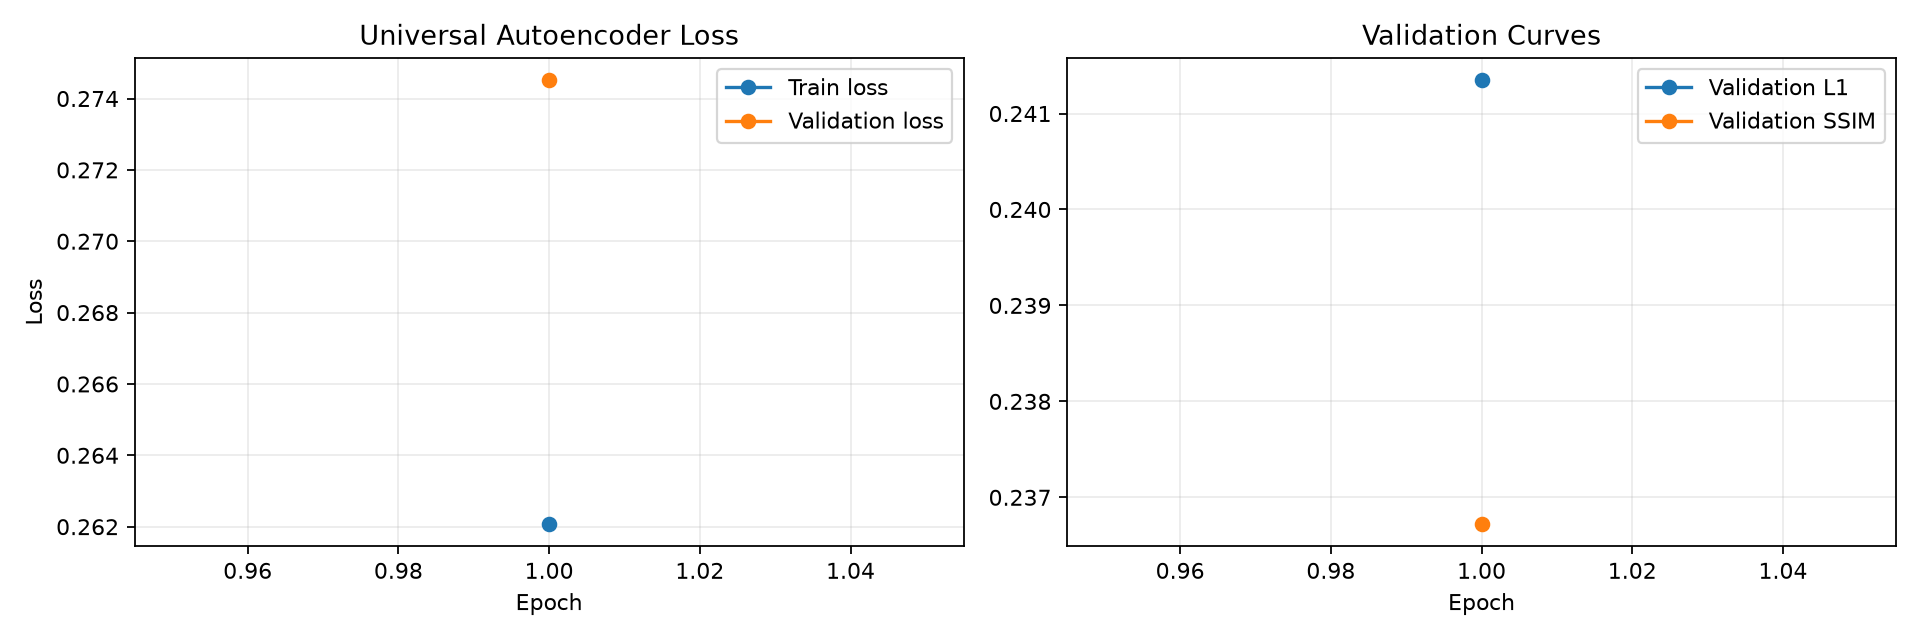
\includegraphics[width=\columnwidth]{task1_final_training_curves.png}
\caption{Task 1 training and validation curves recorded by the final training script.}
\label{fig:task1-curves}
\end{figure}

\section{Task 2: Hard-Routed Restoration}
\subsection{Classifier}
The classifier predicts four classes: clean, salt-and-pepper, blur, and occlusion. Labels are generated by the runtime corruption pipeline. An exact balanced batch sampler supplies equal class counts in every full batch. The classifier uses convolutional blocks, adaptive pooling, dropout, and a four-logit output trained with cross-entropy.

Optuna investigated learning rate, batch size, channel configuration, dropout, and weight decay. Three trials were completed. The best recorded validation accuracy was 0.25, macro precision 0.1833, macro recall 0.25, and macro F1 0.1421. The best parameters were learning rate $2.7036\times10^{-4}$, batch size 16, channels $(48,96,192)$, dropout 0.39259, and weight decay $3.9721\times10^{-6}$.

\subsection{Specialists and Routing}
Three independently parameterized autoencoders restore salt-and-pepper, blur, and occlusion inputs. In hard routing, a predicted clean class uses an identity bypass; otherwise the corresponding specialist is selected. Oracle routing uses the known deterministic corruption label and predicted routing uses the classifier output.

On 80 deterministic test samples, oracle routing produced loss 0.40987, L1 0.21087, and SSIM 0.36639. Predicted routing produced loss 0.45541, L1 0.23430, and SSIM 0.29599. Classifier accuracy was 0.30, with 56 routing mistakes. The largest operational failures occurred when clean images were incorrectly routed to the blur expert, replacing identity output with an unnecessary restoration transformation.

\section{Task 3: Soft Mixture-of-Experts}
The soft model contains a gate, an identity branch, and the three Task 2 specialists. For temperature $\tau$, the gate computes
\begin{equation}
w=\mathrm{softmax}(G(x_c)/\tau),
\end{equation}
and the reconstruction is
\begin{equation}
\hat{x}=w_cx_c+w_sA_s(x_c)+w_bA_b(x_c)+w_oA_o(x_c).
\end{equation}
The gate and experts are initialized from Task 2. Experts are frozen during a gate warm-up and then unfrozen for joint fine-tuning at a smaller learning rate.

The joint loss is
\begin{equation}
L_{joint}=\lambda_{rec}L_1+\lambda_{ssim}(1-SSIM)+\lambda_{cls}L_{CE}+\lambda_{bal}L_{balance}.
\end{equation}
The balance term penalizes the squared distance between batch-average routing weights and a uniform four-branch target. Optuna investigated the four loss weights, temperature, and joint learning rate. The best three-trial configuration was $\lambda_{rec}=1.74866$, $\lambda_{ssim}=0.81851$, $\lambda_{cls}=0.09909$, $\lambda_{bal}=0.000403$, $\tau=0.78242$, and joint learning rate $1.1208\times10^{-5}$. The best recorded joint loss was 0.82529.

Routing analysis across 80 samples found average weights Clean 0.2451, Salt 0.2351, Blur 0.2645, and Occlusion 0.2553. No expert fell below the inactivity threshold of 0.05. Every evaluated sample had multiple contributing branches, and no sample had a single branch above 0.5. Heatmaps, distributions, dominant examples, and multi-expert examples were generated for the report.

\begin{figure}[t]
\centering
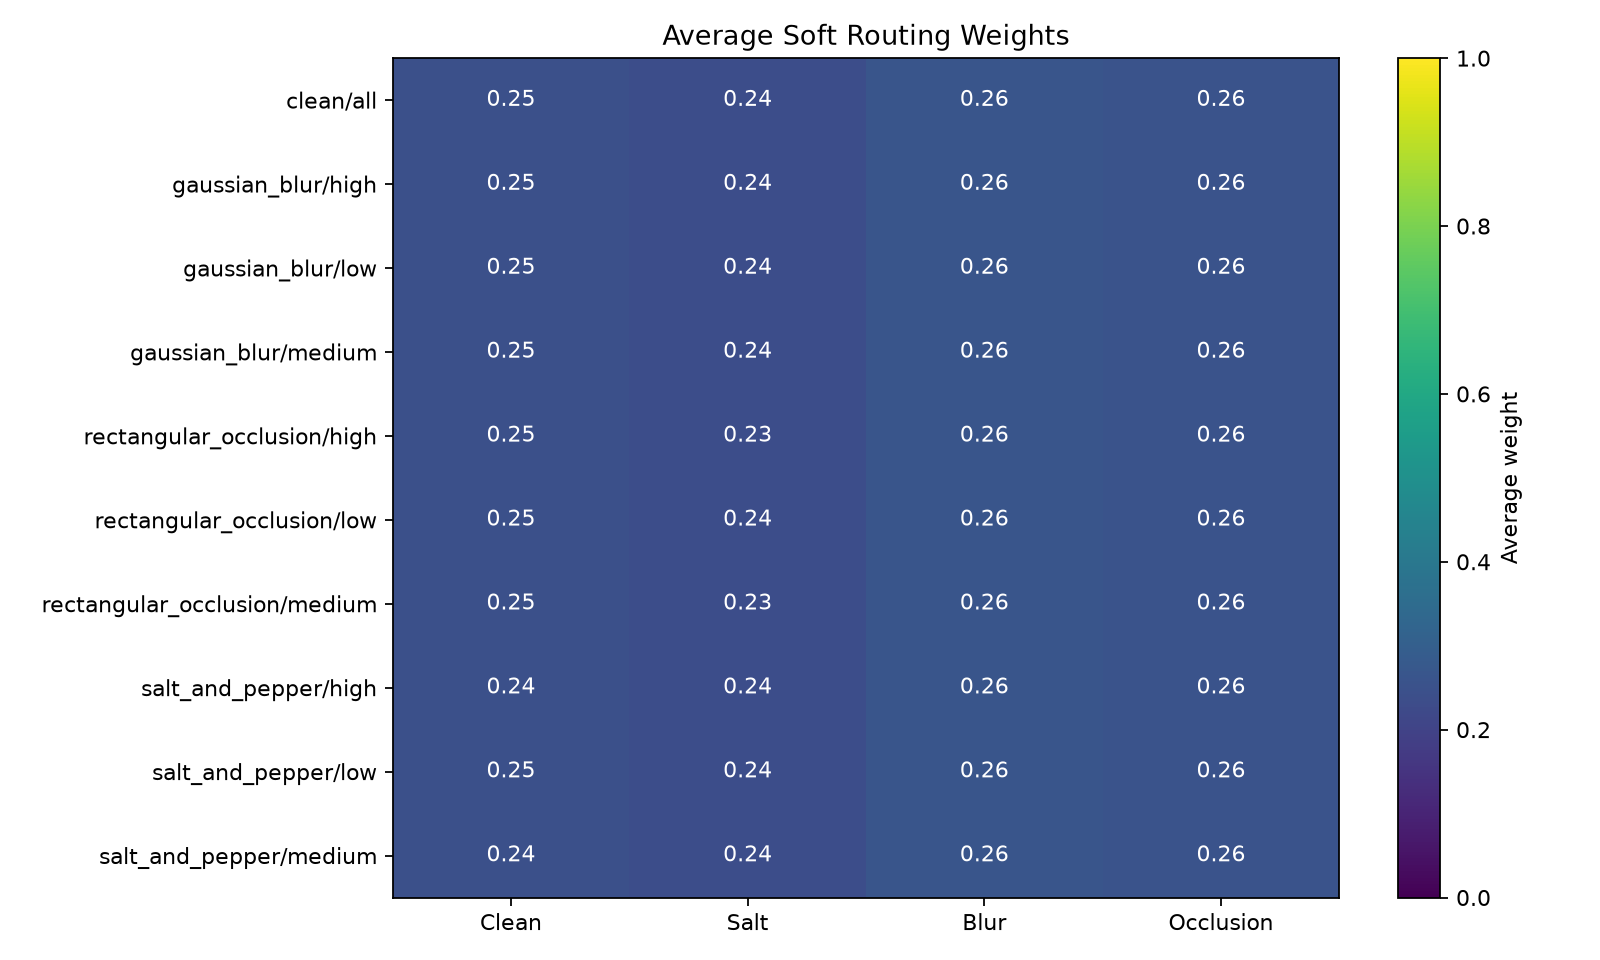
\includegraphics[width=\columnwidth]{task3_routing_analysis/routing_heatmap.png}
\caption{Average soft routing weights by corruption and severity.}
\label{fig:routing-heatmap}
\end{figure}

\section{Task 4: Conditional Face-to-Sketch GAN}
\subsection{Generator}
The generator is a U-Net-style encoder-decoder. A learned embedding maps each of the three style IDs to a vector, projects it to a spatial feature map, and concatenates it with the image bottleneck. Thus, the style condition affects the generated sketch rather than only the user interface.

\subsection{Discriminator}
The discriminator is a PatchGAN. It receives the photograph, candidate sketch, and a spatially broadcast learned style embedding. Its output is a grid of local real/fake logits, encouraging locally plausible sketch structure.

\subsection{Training and Loss}
The generator objective is
\begin{equation}
L_G=L_{adv}+\lambda_{rec}\|y-G(x,s)\|_1,
\end{equation}
while the discriminator uses real and fake binary cross-entropy with logits. The assignment's $\lambda_{rec}=100$ is treated as an initial value; the implementation exposes an Optuna search range of 10--200 on a log scale. The final CPU smoke-training run used $\lambda_{rec}=100$, batch size 2, $128\times128$ images, and one bounded epoch.

Recorded losses were discriminator real 0.84018, discriminator fake 0.58253, generator adversarial 0.72045, and generator reconstruction 0.84762. Validation L1 was 0.84579 and validation adversarial loss was 0.61423. Generated validation samples were saved for style-conditioned inspection.

\begin{figure}[t]
\centering
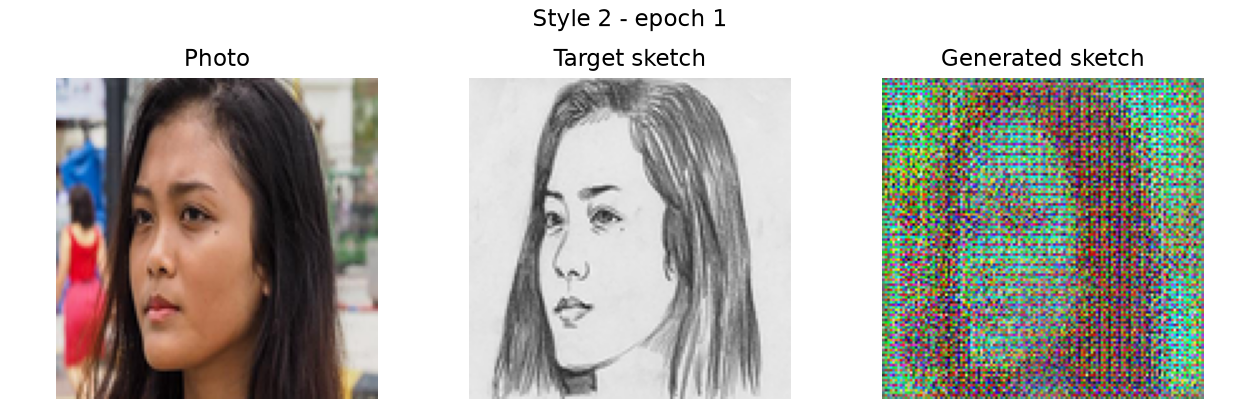
\includegraphics[width=\columnwidth]{task4_generated_validation_samples/epoch_001_sample_00.png}
\caption{Example validation output containing photograph, target sketch, and generated sketch.}
\label{fig:gan-sample}
\end{figure}

\section{Experimental Setup}
The implementation uses Python 3.14, PyTorch, torchvision, NumPy, Pillow, OpenCV, scikit-image, scikit-learn, Optuna, ONNX, and ONNX Runtime. Seeds are recorded as 42 where applicable. The primary development device was CPU, which motivated bounded trial and training budgets. All model checkpoints and JSON reports are stored under the repository's task, report, and checkpoint directories.

\section{Results}
Table~\ref{tab:results} summarizes the main recorded results. These values are experiment artifacts rather than claims of fully converged large-scale training because the report explicitly preserves the batch and epoch caps used in the development environment.

\begin{table}[t]
\centering
\caption{Recorded validation results.}
\label{tab:results}
\begin{tabular}{lccc}
\toprule
System & Loss & L1/Accuracy & SSIM/Macro F1 \\
\midrule
Universal & 0.28047 & 0.25001 & 0.27061 \\
Hard oracle & 0.40987 & 0.21087 & 0.36639 \\
Hard predicted & 0.45541 & 0.23430 & 0.29599 \\
Classifier & -- & 0.25000 & 0.14211 \\
Soft MoE & 0.82529 & 0.15624 & -- \\
GAN validation & -- & 0.84579 & -- \\
\bottomrule
\end{tabular}
\end{table}

\subsection{ONNX Consistency}
All deployed models were checked with ONNX Runtime. Task 1's maximum output difference was $1.19\times10^{-7}$. Task 2's classifier maximum difference was $1.86\times10^{-9}$ and each expert was $1.19\times10^{-7}$ or lower. The Task 3 restored-image maximum difference was $1.19\times10^{-7}$ and routing weights matched exactly. The Task 4 generator was checked for all style IDs; the largest difference was $8.42\times10^{-6}$, within $\mathrm{atol}=10^{-5}$ and $\mathrm{rtol}=10^{-4}$.

\section{Application Architecture}
The application consists of a React/Tailwind frontend, a FastAPI backend, ONNX Runtime sessions, and Docker Compose. The frontend provides Home, Universal Restoration, Hard-Routed Restoration, Soft MoE Restoration, and Face-to-Sketch workspaces. The backend validates image type and size, decodes and resizes inputs, loads cached ONNX sessions, performs inference, postprocesses outputs, and returns base64 PNG data plus timing and routing metadata.

The backend exposes $/health-check$, $/universal-restoration$, $/hard-routing$, $/soft-mixture$, and $/face-to-sketch$. The face-to-sketch endpoint accepts style IDs 0--2. The container stack uses an Nginx frontend image and a Python FastAPI backend image; Compose waits for backend health before starting the frontend dependency. The documented command is \texttt{docker compose up --build}.

\section{Limitations}
The most important limitation is compute budget. Several Optuna studies used three trials and bounded batches, and final model artifacts were smoke-trained for limited epochs. Consequently, the reported metrics should be read as reproducible implementation checkpoints, not as a final benchmark against fully converged training. The classifier's low accuracy demonstrates a second limitation: routing errors can dominate restoration quality, especially for clean inputs that should have used identity bypass. The soft gate was also diffuse in the analyzed checkpoint, so it did not yet demonstrate sharp expert specialization. The GAN requires further multi-epoch training and a completed Optuna sweep on the full prepared validation set. Finally, the frontend is a functional workspace shell; production deployment would require wiring its controls to the FastAPI endpoints, authentication, request queues, and persistent experiment tracking.

\section{Conclusion}
This work implements a complete progression from universal restoration to hard routing, soft mixtures, and style-conditioned face-to-sketch synthesis. The systems share deterministic data preparation, explicit losses, Optuna configuration records, checkpoint artifacts, ONNX export, and an inference application architecture. The experiments show the value of a clean identity bypass and expose the cost of weak classification in a hard-routing system. Future work should use longer GPU-backed training, broader Optuna studies, improved classifier data augmentation, and full frontend-to-backend interaction testing.

\section*{AI-Use Appendix}
Generative AI assistance was used as a programming collaborator for repository scaffolding, implementation drafts, debugging, test design, experiment bookkeeping, and technical writing organization. The human author selected the assignment interpretation, reviewed and modified generated code, ran the experiments, inspected failures, and verified model outputs, ONNX consistency, dataset preparation, and container configuration. AI-generated suggestions were not treated as experimental evidence; numerical results in this paper come from the recorded workspace artifacts and executed validation checks.

\begin{thebibliography}{00}
\bibitem{wang2004ssim} Z. Wang, A. C. Bovik, H. R. Sheikh, and E. P. Simoncelli, ``Image quality assessment: From error visibility to structural similarity,'' \emph{IEEE Trans. Image Process.}, vol. 13, no. 4, pp. 600--612, 2004.
\bibitem{ronneberger2015unet} O. Ronneberger, P. Fischer, and T. Brox, ``U-Net: Convolutional networks for biomedical image segmentation,'' in \emph{Proc. MICCAI}, 2015, pp. 234--241.
\bibitem{isola2017pix2pix} P. Isola, J.-Y. Zhu, T. Zhou, and A. A. Efros, ``Image-to-image translation with conditional adversarial networks,'' in \emph{Proc. CVPR}, 2017, pp. 1125--1134.
\bibitem{fan2022fs2k} D.-P. Fan, Z. Huang, P. Zheng, H. Liu, X. Qin, and L. Van Gool, ``Facial-sketch synthesis: A new challenge,'' \emph{Machine Intelligence Research}, 2022.
\bibitem{fs2k} D.-P. Fan and P. Zheng, ``FS2K Facial Sketch Synthesis Dataset,'' GitHub repository, 2021. [Online]. Available: \url{https://github.com/DengPingFan/FS2K}
\bibitem{onnx} Open Neural Network Exchange, ``ONNX documentation.'' [Online]. Available: \url{https://onnx.ai/}
\bibitem{optuna} T. Akiba, S. Sano, T. Yanase, T. Ohta, and M. Koyama, ``Optuna: A next-generation hyperparameter optimization framework,'' in \emph{Proc. KDD}, 2019, pp. 2623--2631.
\end{thebibliography}

\end{document}
